\section{Localization in the Presence of Authorized Users}
\label{sec:authorized}

Till now, we have assumed that the only transmitters present in the area are the intruders which need to be localized. In this section, we solve the more general \mtl problem, where there may be a set of authorized users in the background. 
This is referred to as the multiple transmitter localization - shared spectrum (\mtlss) problem \cite{ipsn20-mtl}.

In particular, in a shared spectrum paradigm, there are primary users and an evolving set of active secondary users transmitting in the background.
Different than the intruders whose locations are unknown, the authorized users' locations are known and we wish to utilize this known information to better localize the unknown intruders.
The key challenges come from the fact that the set of authorized users is not static and changes over time as allocation requests are granted and/or active secondary users become inactive over time.
A straightforward way to handle background authorized users is to localize every transmitter, and then remove the authorized users. 
However, any localization approach is susceptible to performance degradation with the increase in the number of transmitters to be localized.
Thus, the straightforward approach of localizing every transmitter is likely to be error-prone.
Therefore, we attempt to develop a new approach that uses \our as a building block that uses the information of the location of the authorized uses in a way other than removing them after localizing all.
The new approach tries to subtract the received signal strength at the sensors by a value received from the authorized users.
This subtraction is done by a novel CNN model; we refer to it as \subtract.
Then we feed the image with subtracted powers to the \our and get the locations of the intruders.
See Fig.~\ref{fig:subtractnet}(c)--(d)--(f).
We describe \subtract in the following paragraphs.

% \begin{figure}
%     \centering
%     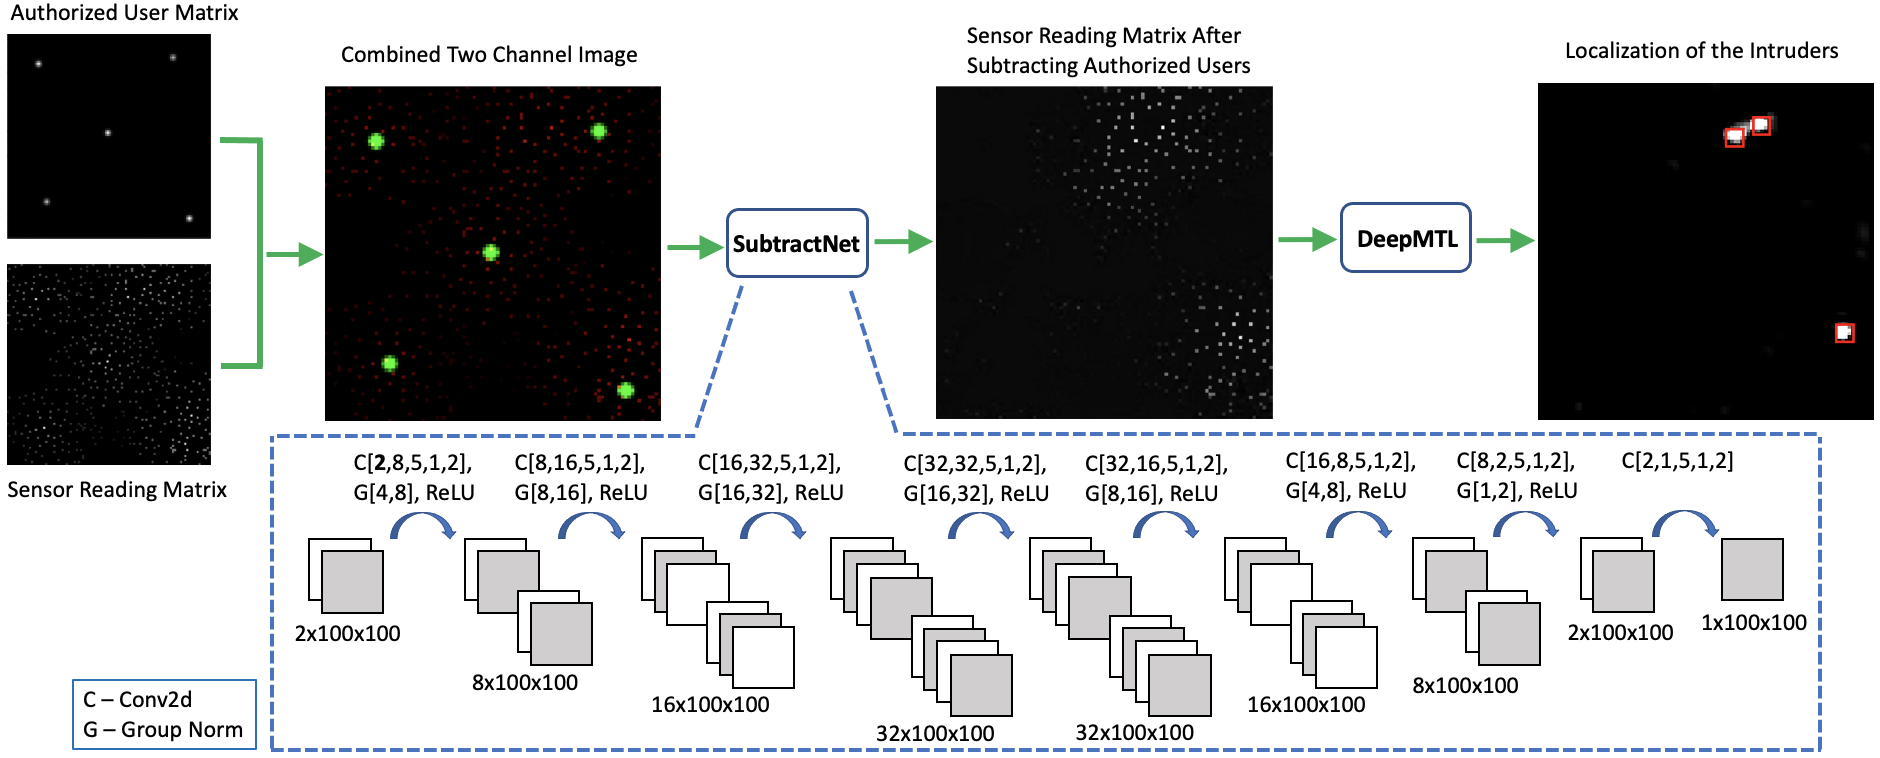
\includegraphics[width=\textwidth]{figures/subtractnet.png}
%     \caption{Overall architecture of second approach to localize 3 intruders in the presence of 5 authorized users (in color green). The details of the \subtract model is in the dotted box.}
%     \label{fig:subtractnet}
% \end{figure}

\begin{figure}
    \centering
    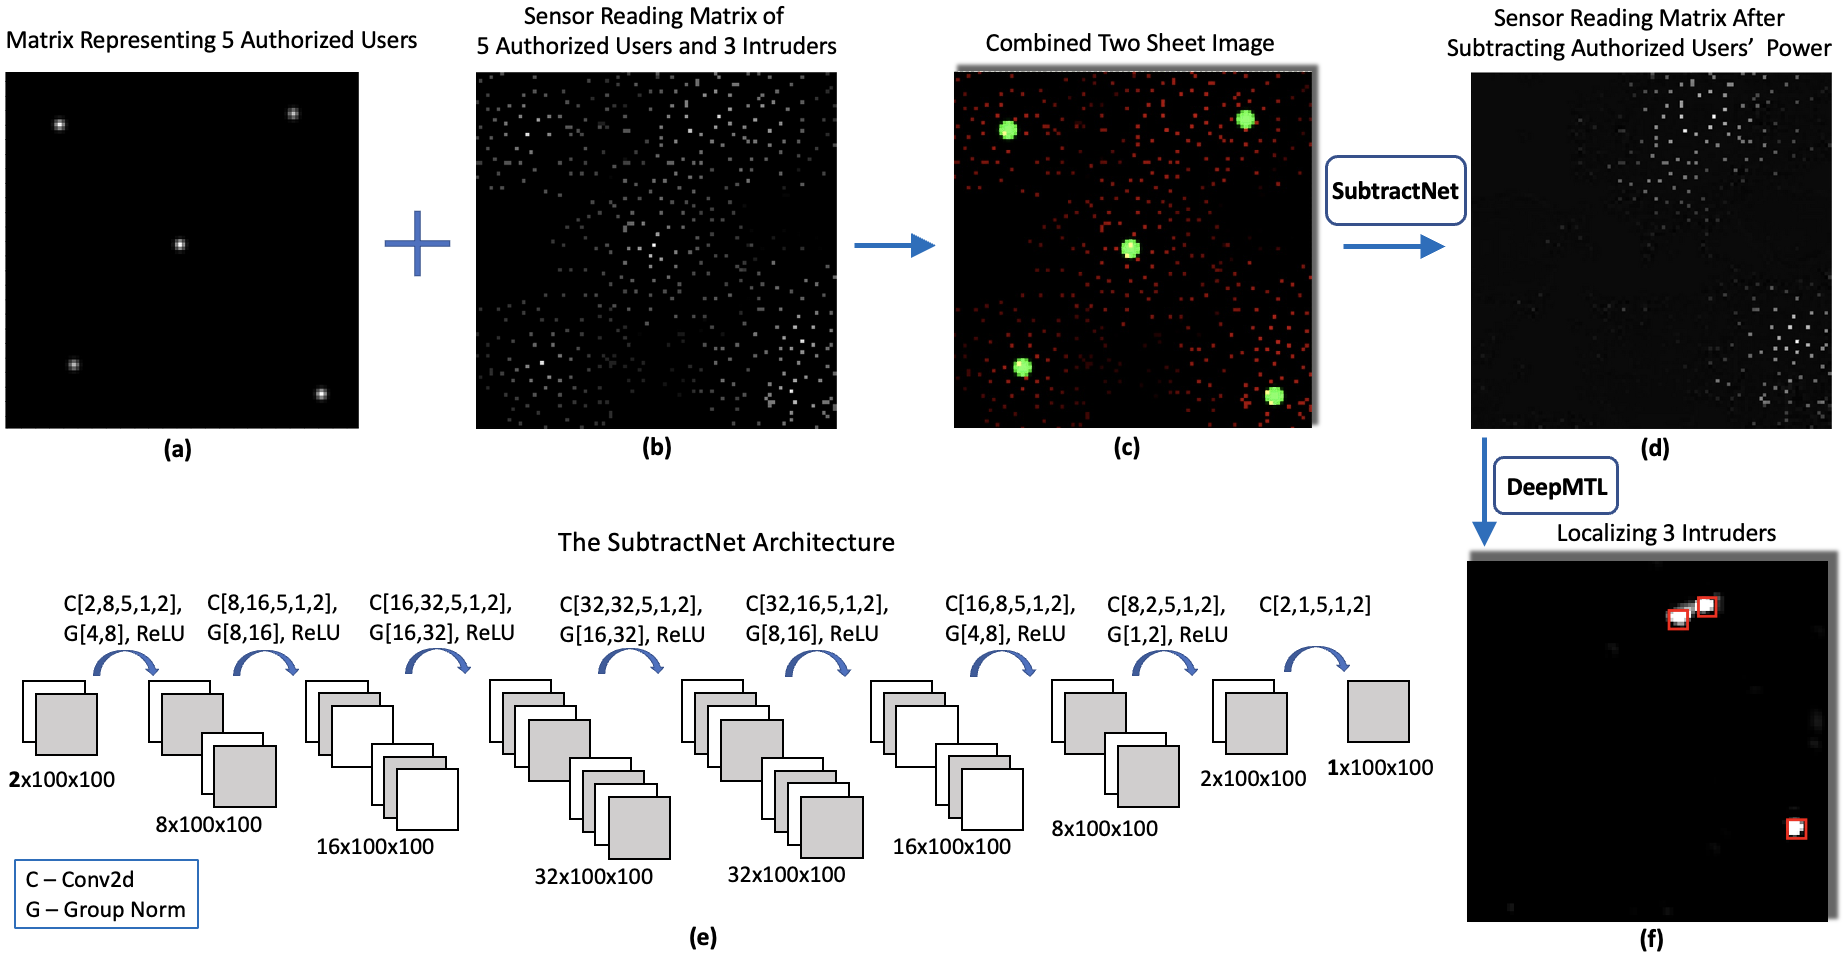
\includegraphics[width=\textwidth]{chapters/wowmom-pmc/figures/subtractnet2.png}
    \caption{Overall architecture of second approach to localize 3 intruders in the presence of 5 authorized users. The input of the \subtract is (c), which is stacking authorized user matrix (a) and the sensor reading matrix (b). (d) is the output of \subtract, where the transmission power of the authorized users is subtracted from the area. The details of the \subtract model is in (e). (f) is the localization output after feeding (d) into \our.}
    \label{fig:subtractnet}
\end{figure}

\softpara{\subtract Input Image}. The sensor reading has two sources, one is the intruders and the other is the authorized users.
We aim to subtract the power of the authorized users and remain the power from the intruders.
So the input of the \subtract will contain two kinds of information: the authorized users' information (Fig.~\ref{fig:subtractnet}(a)), including both the location and the transmitter power, and the sensor reading matrix (Fig.~\ref{fig:subtractnet}(b)) that encode the power from all transmitters.
To incorporate the two kinds of information, we first encode the authorized user information into a matrix that has the same dimension as the sensor reading matrix.
Then stack the two matrices together.
The combined stacked image is nothing but a two-channel image, which can be interpreted as Red and Green channels.
The sensor reading matrix is the Red channel and the authorized user matrix is the Green channel. There is no Blue channel.
To represent the authorized transmitter in the Green channel, we use a Gaussian peak similar to what we did in the \imgimg for representing transmitters (Section \ref{sec:translate}).
The difference is that in \imgimg, all the peaks have a uniform height, whereas in \subtract, the height of the peak is the power of the authorized transmitter.
So the higher the power of the authorized transmitter, the higher the peak in the Green channel.
Another difference is that the authorized transmitters are approximated at discrete locations instead of the continuous locations as in \imgimg.

\softpara{\subtract Output Image}. 
The \subtract's output image is just a one-channel images and represents the sensor readings due to the intruders only.  

\softpara{\subtract CNN Architecture}.
We refer to the model that subtracts the power from the authorized users as the \subtract. 
It has a similar design philosophy with \imgimg.
\subtract is also an image-to-image translation neural network.
Compared to \imgimg, it doubled the number of layers, mainly because \subtract needs a bigger receptive field than \imgimg.
A bigger receptive field can let the CNN model update sensors that are further away from the authorized user.
For the loss function, we use the L2 loss function, similar to the loss function used in Equation~\ref{equ:sen2peak_loss}, merely replacing the \imgimg with \subtract in Equation~\ref{equ:sen2peak_loss}.
The training details are also the same as in \imgimg.
